\documentclass[class=book, crop=false, 11pt]{standalone}
\usepackage[subpreambles=true]{standalone}
\usepackage[utf8]{inputenc}
\usepackage{import}
\usepackage[ruled,vlined]{algorithm2e}

\usepackage{amsmath}
\usepackage{amssymb}
\usepackage[margin=1.2in]{geometry}
\usepackage[sorting = none,
            doi = true  %lesedato for url-adresse
            ]{biblatex} %none gir bibliografi i sitert rekkefølge
\addbibresource{reference.bib}
\usepackage{csquotes}
\usepackage{pgfplots}
\usepackage{pgfplotstable}
\usepackage[font=small,labelfont=bf]{caption}


\pgfplotsset{compat=1.15}

\begin{document}
\chapter{Discussion}\label{chapter:discussion}
\section{Nominal values for consumption and production}
The action of the reinforcement agent determines the percentage change in demand at each load in the interval $[-f,f]$, where $f$ is the flexibility of demand. Naturally, the load is varying a lot throughout a day, but the nominal demand also vary a lot from bus to bus. Figure \ref{fig:discussion:nominal_load} shows the values for nominal apparent power at each bus bar in the power system, as predefined in \texttt{pandapower}.

\begin{figure}[ht]
    \center
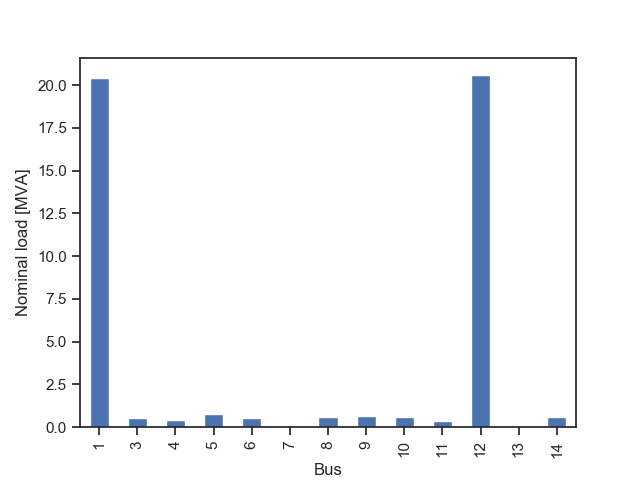
\includegraphics[height=8cm, width=12cm]{figures/nominal_load.png}
    \caption[size = 9]{Bar plot of the nominal apparent power at each bus in the CIGRE network}
    \label{fig:discussion:nominal_load}
\end{figure}

Bus 1 and 12 clearly stand out, and account for nearly 90 \% of the total system demand. For simplicity, they will be referred to as the dominant buses due their large demand. Note that there is no solar power connected to them. Because each action variable is scaled up by the nominal load, it is clear that action +1 for the dominant buses has a much larger impact in terms of absolute power change than it has on the rest of the buses. As shown in figure \ref{fig:discussion:cigre_network_dominant}, The dominant buses are placed in the top of each feeder 1 and feeder 2, connected to each their 220/22 kV transformer. 

\begin{figure}[ht!]
    \center
    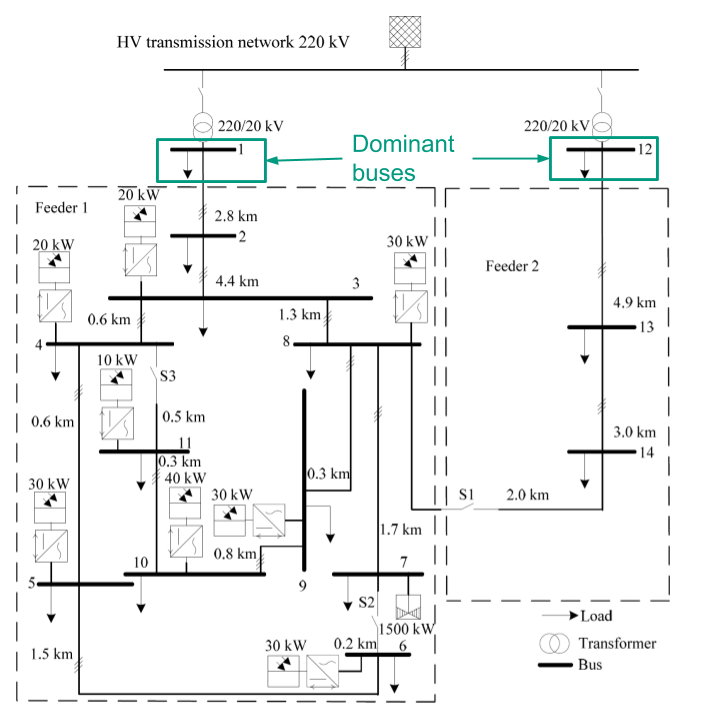
\includegraphics[height=14cm, width=13.5cm]{figures/cigre_network_dominant.png}
    \caption[size = 9]{CIGRE network with solar and wind power that is used in the reinforcement learning algorithm \cite{cigre}. The dominant buses account for approximately 90 \% of the power consumption in the grid}
    \label{fig:discussion:cigre_network_dominant}
\end{figure}
It might seem troubling that the dominant buses have much larger nominal values. However, because they are placed next to the grid, they do not affect the line current in the rest of the system much. For instance, if the consumption at bus 1 is doubled, the current through the transformer approximately doubles to supply the demand. Naturally, this could be very critical for the transformer, but it has a small effect on the line currents in the power system, because the rest of the loads still draw the same amount of power from the grid. The line current effect of changing the demand at bus 1 and 12 are not that decisive as one first might think, due to their position close to the external grid. On the other hand, they can greatly affect the voltage magnitudes in the grid. Figure \ref{fig:discussion:double_large_load} illustrates the effect increasing the demand at the dominant buses has on the rest of the buses. The predefined demand values are used for solving the power flow equations in situation A, while they are doubled for the dominant buses (1 and 12) in situation B, leaving the other buses unchanged.

\begin{figure}[ht!]
    \center
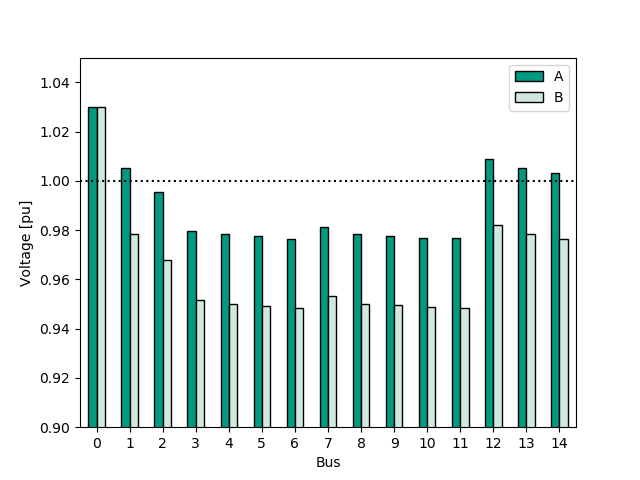
\includegraphics[height=8cm, width=12cm]{figures/double_large_load.png}
    \caption[size = 9]{Bar plot for each of the buses showing their voltage magnitude in nominal operation (A) and after the demand at bus 1 and 12 in figure \ref{fig:discussion:cigre_network_dominant} are doubled (B). Note that the vertical axis is truncated}
    \label{fig:discussion:double_large_load}
\end{figure}
The dominant buses serve as the starting point for the voltage magnitudes because they are at the beginning of the two feeders. This is true because there are only PQ-buses in the system and no voltage regulating units. The voltage is static at the external grid, and gradually falls as we move down the feeders in periods of peak demand. The voltage magnitude at bus 1 is reduced when it doubles its demand, which in turn propagates down the feeder and affects all buses in the feeder. The reinforcement agent is not allowed to double the demand in the reinforcement algorithm, but figure \ref{fig:discussion:double_large_load} illustrates the decisive effect of the dominant buses in terms of voltage magnitudes.

\begin{figure}[hb!]
    \center
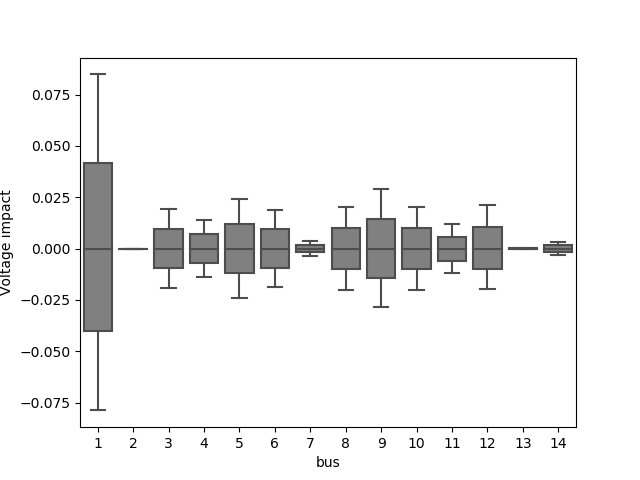
\includegraphics[height=8cm, width=12cm]{figures/voltage_impact.png}
    \caption[size = 9]{Box plot for each bus bar showing the voltage impact for a flexibility of demand ranging from -20 to + 20 \% in an hour of peak demand}
    \label{fig:discussion:voltage_impact}
\end{figure}

A measure of impact is needed to systematically investigate the effects of changing the demand at a bus. Let the voltage and current impact of a bus respectively be defined as the sum of the changes in voltage and current loading in the net when modifying the demand at that bus by a certain percent. Note that the rest of the buses are left unchanged when calculating the impact. For instance, the voltage impact of bus 1 and 12 of in figure \ref{fig:discussion:double_large_load} is the voltage difference of scenario A and B, summed over all buses. The same can be done for the current impact, which is the difference in current loading summed over all lines. The current loading in a line is a percentage of the line capacity, not ampere. The current impact is therefore weighted against the capacity of the line. The impact of a bus will be discussed for the two critical periods of the day, namely peak solar production and peak demand. For peak solar production, the average demand and maximum solar production at 12 am during the 500 episode test simulation are used to define the values for consumption and production. For peak demand, the average solar production and maximum demand at 8 pm are used. 


Figure \ref{fig:discussion:voltage_impact} plots the voltage impact during peak demand for each bus where the demand change ranges from -20 to +20 \%. The lower part of the box plots correspond to increasing the demand by 20 \%, since increasing the consumption in peak demand lowers the voltage magnitudes in the grid. As already discussed, bus 1 has a large voltage impact, because it is at the top of feeder 1. 


Figure \ref{fig:discussion:current_impact} plots the current loading impact in peak demand hours for the buses in the net, where the demand change ranges from -20 to +20 \%. The lower part of the box plots corresponds to decreasing the consumption by 20 \%, since less current is needed to supply the demand. The buses with highest current impact (5, 6, 9, 10) are all located far down in feeder 1. A change in demand at them has consequences for several lines, because the current they draw must travel through the lines in the top of the feeder. As discussed, the current loading impact is low for the dominant buses (1 and 12), despite the fact that they account for nearly 90 \% of the consumption in the system. 


\begin{figure}[h]
    \center
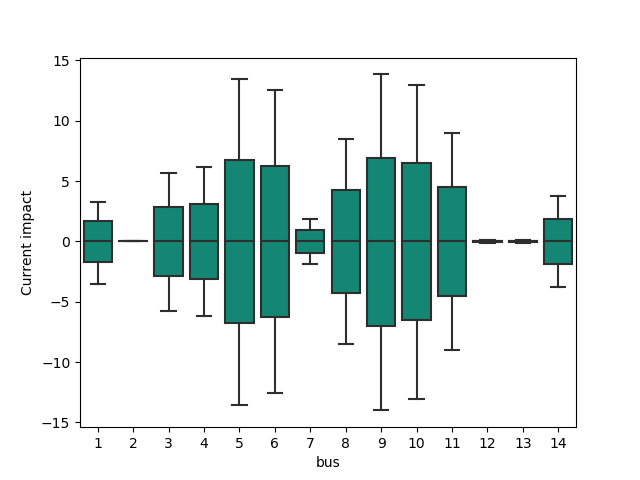
\includegraphics[height=8cm, width=12cm]{figures/current_impact.png}
    \caption[size = 9]{Box plot for each bus bar showing the current impact during peak demand for a demand change ranging from -20 to + 20 \%}
    \label{fig:discussion:current_impact}
\end{figure}

So far the impacts of the buses have been investigated in hours of peak demand. A similar simulation in an hour of peak solar production can be done to show the impact of the buses in the second critical period. The impact relation between the buses in peak solar hours is similar to the peak demand period. In other words, if a bus has a large impact in peak demand, it also has large impact during peak solar production compared to the other buses. However, the magnitude differs a lot for the two critical periods. Figure \ref{fig:discussion:current_impact_demand_solar} plots the current loading impact factor for each bus when the demand is increased by 10\% in hours of peak demand and peak solar production. The current impacts in peak solar production are lower in all cases, except for bus 1. Similarly, figure     \ref{fig:discussion:voltage_impact_demand_solar} show the difference in voltage impact during peak demand and peak solar production. The impacts differ because the power consumption generally is lower during peak solar production. The mean demand during maximum solar production at 12 am is less than half of the max demand value at 7 pm. Consequently, changing the demand by 10 \% at 12 am results in a absolute power change that is about half the change during peak demand. The agent simply has less muscles during peak solar production, because it is physically impossible to affect the grid as much as in the afternoon during peak demand. This can explain why the trained agent performs well i periods of peak demand and poorly in periods of peak solar production.

\begin{figure}[h]
    \center
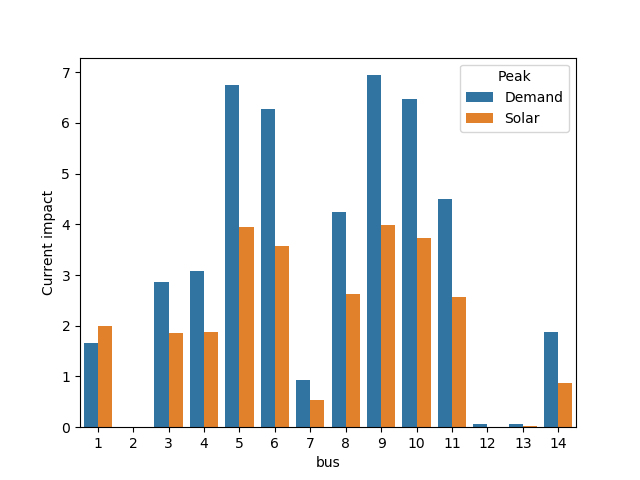
\includegraphics[height=8cm, width=12cm]{figures/current_impact_demand_solar.png}
    \caption[size = 9]{Current impact of all the buses in an hour of peak demand and peak solar production. The demand is changed by 10 \%}
    \label{fig:discussion:current_impact_demand_solar}
\end{figure}

\begin{figure}[h]
    \center
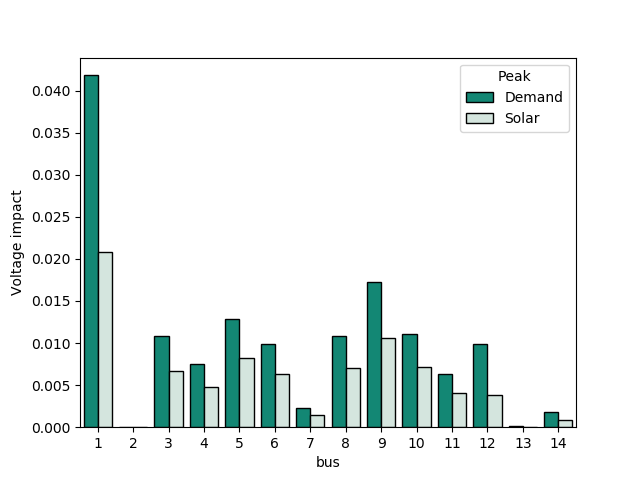
\includegraphics[height=8cm, width=12cm]{figures/voltage_impact_demand_solar.png}
    \caption[size = 9]{Voltage impact of all the buses in an hour of peak demand and peak solar production. The demand is changed by 10 \%}
    \label{fig:discussion:voltage_impact_demand_solar}
\end{figure}

\section{Performance of the trained agent}
The results from section \ref{section:result:config1} show that the trained agent is able to reduce the number of safety violation by 10\%. However, the trained agent is only able to reduce violations of voltage safety margins, not current violations. In fact, it increases the number of current violations by 18 \%. Still, there are large differences in terms of the quantity and magnitude of the current and voltage safety violations. There are almost 7 times more voltage violations than current violations. This is of course dependent on the voltage bounds that are used for defining the voltage cost, which in this case are 0.95 and 1.05 pu. Although there are many more voltage violations in a normal day, the average current violation is more severe. Specifically, the mean current cost is almost 5 times greater than the mean voltage cost. The nature of the transmission in terms of violations is therefore: the current violations are sparse and severe, while the voltage violations are numerous and faint. 

Why is the trained agent better at avoiding voltage violation than current violations? A possible reason is that the agent is penalised more for voltage violations on average. The total voltage cost is 40 \% greater than the total current cost, because they are more frequent. It is sensible that the agent learns a behaviour that reduces the most punishing term, namely the voltage cost. As stated in section \ref{section:config1:current_violations}, the trained agent only learned the appropriate behaviour in periods of peak demand. This can be explained by the time of the day the voltage violations occur. There are 80 \% more voltage violations during peak demand than during peak solar production. In other words, voltage violations are the most punishing term and they are most frequent in the afternoon. Imagine that the agent has the correct behaviour in the beginning of training, i.e that it increases consumption during peak solar and decreases it during peak demand. The agent will experience a greater boost in reward by behaving correctly in peak demand, because then the voltage cost is highest. Put differently , it is easier for the agent to learn the correct behaviour during peak demand. It is natural that the agent first focuses on the low-hanging fruits, and decreases the power demand. 

\begin{figure}[h]
    \center
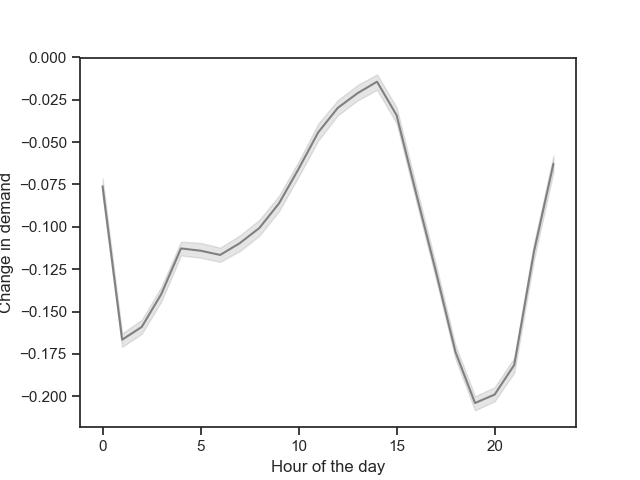
\includegraphics[height=8cm, width=12cm]{figures/config1_action_hour.png}
    \caption[size = 9]{Hourly mean values for the change in demand at the buses in the net, as determined by the trained reinforcement agent. The error region is a 95 \% confidence interval of the mean value}
    \label{fig:discussion:config1_action_hour}
\end{figure}

The agent was worsening the situation in periods of peak solar production. The desired behaviour in such a situation is to increase the demand, so that less excess solar power needs to be exported to the grid. However, the trained agent decreases the demand in periods of peak solar production, since the number of line overload increases. It is possible that the learned behaviour simply is to decrease the demand at all times, especially when considering that the energy imbalance in the system is negative, as shown in figure \ref{fig:results:configuration1_energy_imbalance}. Figure \ref{fig:discussion:config1_action_hour} shows the mean action taken by the agent throughout a the day in the 500 episode simulation, with a 95 \% confidence interval. The pattern of the actions is as desired, because it goes up during peak solar producing and down during peak demand in the afternoon. However, the change in demand during peak demand is still negative. The action signal seems to have a negative bias. It is also worth noting that the mean action is quite low in absolute magnitude. In other words, the agent is not synchronising the buses such that the entire available flexibility in the system used.

\begin{figure}[h]
    \center
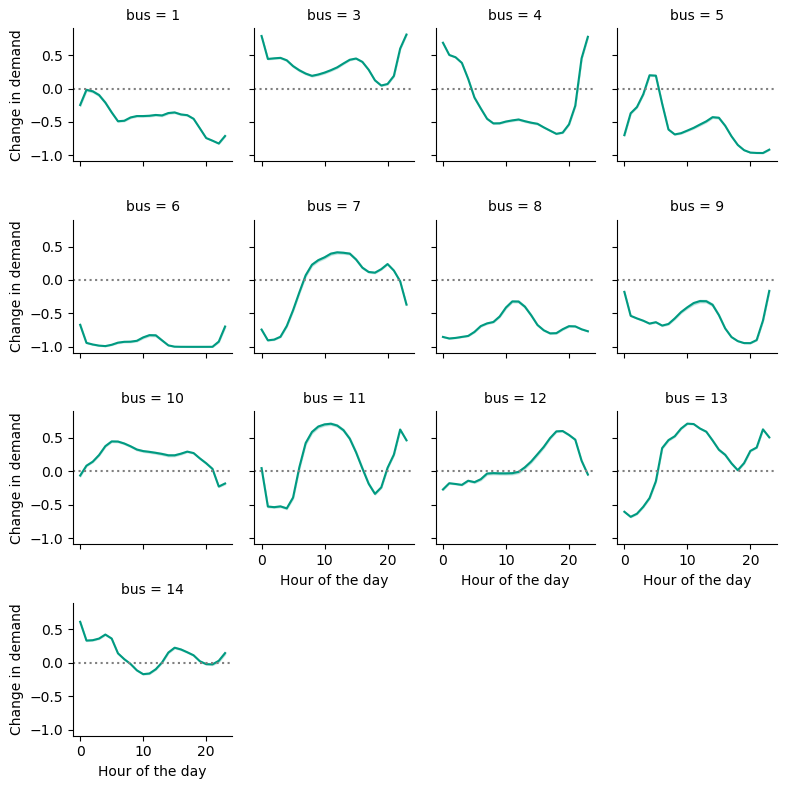
\includegraphics[height=13cm, width=12cm]{figures/config1_action_bus.png}
    \caption[size = 9]{Hourly mean values for the change in demand in the net for each bus, as determined by the trained reinforcement agent. The error region is a 95\% confidence interval}
    \label{fig:discussion:config1_action_bus}
\end{figure}

Figure \ref{fig:discussion:config1_action_bus} shows mean values for demand change throughout a day for each bus.  The buses 1, 6, 8 and 9 are on average negative in every hour, i.e the agent always reduces the consumption. As discussed, the different buses have different voltage and load current impact, and it is interesting to see whether there is a relationship between actions and load current/voltage impact of the buses. First it can be noted that bus 1 (top left corner) which has the largest voltage impact in hours of peak demand mainly is negative in an average day. This can suggest that the trained agent has learned that lowering the consumption is beneficial in peak demand hours, and therefore has a strong negative bias that pulls the demand change to negative values throughout the day. The buses with strongest current impact are 5, 6, 9 and 10, and they do not show a particular desired pattern. Only bus 10 increases the power consumption during peak solar. Bus 9, which has a high current and voltage impact, has a reasonable curve shape, but it is negatively biased which results in a decrease in power consumption in all hours. Perhaps the most sensible mean action signal is for bus 11. Still, there is no obvious pattern that suggests that the trained agent has learned a particularly well-coordinated behaviour. It might very well be that it is the agent's negative bias, i.e its tendency to always decrease power consumption, that leads to less voltage violations in the grid.

\section{Solar power production}
The nominal solar production level predefined in the network is scaled up by a factor of 40. This is done to challenge the grid by increasing the number of current and voltage violations in hours of peak solar production. The maximum values for solar production and consumption at the solar producing buses are presented in figure \ref{fig:discussion:nominal_sgen}. Naturally, the demand and solar production varies throughout the day. Around maximum solar production, the relation between the mean solar production and mean consumption is similar to the relation showed in figure \ref{fig:discussion:nominal_sgen}. The ratio between solar production and demand at bus 7 is very high, and should probably have been scaled differently than the other buses. The ratio for the rest of the buses ranges from 1.2 to 2.8. 

\begin{figure}[h]
    \center
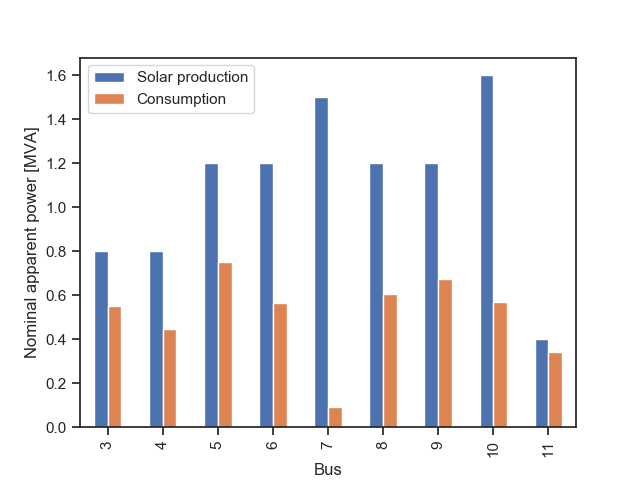
\includegraphics[height=8cm, width=12cm]{figures/nominal_sgen.png}
    \caption[size = 9]{Bar plot of the nominal apparent power consumption and solar production at solar producing buses in the grid}
    \label{fig:discussion:nominal_sgen}
\end{figure}

\section{State representation}
There are many different ways of constructing the state space in the reinforcement agent. In section \ref{section:problem:state_space} several candidates for the state space were introduced, such as the the bus space. The bus space consists of the active power $P$, reactive power $Q$, voltage magnitude $|U|$ and phase angle $\delta$ for all the buses in the system. It was not included in the state space of the trained reinforcement agent. A reason for this is that the bus state in an hour gives limited information about the future. Naturally, there is a correlation between the bus state of the current and next step. For instance, during peak demand in the afternoon, the demand between two hours are highly correlated, which means that the bus states also are correlated. However, this information can be found in the demand forecasts. In some sense, the bus state in the current time step is redundant. During peak solar production, we can have an hour with heavy production from solar units, but in the next hour the forecasts says that there will be cloudy. It is not possible to predict the clouds from the bus state. On the contrary, the agent can be fooled to use the bus state to chose actions, when it really is the forecast is should use, because the predictive information is hidden in the forecast. Of course, the forecasts can be used to predict the next bus state, which can be helpful information for the agent. However, this will slow down the training process, because the power flows equation must be solved, possibly several times if many future bus states are going to be estimated. 

The actions of the agent in a reinforcement learning algorithm interact with the state of the environment. For instance, an agent playing chess can choose to move a pawn based on the state representation of the board. This move directly determines the next board position, and therefore also the next state. The pawn action is very committing since a pawn can not be moved back. The agent must therefore be very farsighted, and be able to estimate future rewards precisely. However, the forecast space used in this thesis is entirely independent of whether the agent increases or decreases the demand power demand at a bus. There's no sophisticated long term planning that the agent can do, because the agent does not affect the next forecast state. The optimal behaviour is to maximise the immediate reward, because the next forecast state will be the same no matter what action is taken. Why would you not take the action that maximises the immediate reward, when your future rewards do not depend on the action? The only state variable the agent influences is the energy imbalance. But the energy imbalance cost is defined by the change in the energy imbalance. Therefore, if the agent takes an action that decreases the energy imbalance in the system, it has little long term consequences for the agent. The agent can in the next time step reduce the consumption again, which results in an even lower energy imbalance. However, since the imbalance cost is independent of the absolute energy imbalance, the agent will be punished equally, regardless of the action it did in the previous step. The arguments for the imbalance scenario are not true when the imbalance is close to zero. Still, the energy imbalance for the trained agent decreased quickly and stabilised at a negative value, so the described scenario is what happens. All in all, there is little long term planning the agent can do. The discount factor ($\gamma \in (0,1)$) in the reinforcement learning algorithm determines how farsighted the agent, and is by default 0.99. It might be more appropriate to lower it, since there's little room for long term planning.  

The agent would however interact with the state variable in an a more realistic modelling of demand response, where there is a direct cost of activating flexibility, and when the future flexibility depends on the actions. If batteries also are included in the system, the agent will affect the future state more than in the experiment analysed in this thesis. A more realistic demand response model would be more like a classical reinforcement learning setup, where the action influences next state which in turn leads to the need for long term planning.

It should be noted that the agent still interacts with the environment, although the forecast state is not affect by the agent's actions. Altering the consumption affects the power flow equations, and therefore the number of violations in the power grid. 


The state space used for training the agent does not include information that is bus specific. The demand, which is expressed as a percentage of nominal power consumption levels at each bus, is assumed equal at every bus. If the demand at a bus is 60 \% of nominal consumption, then the demand at every other bus is also 60 \% of their nominal consumption. Naturally, this is an oversimplification since demand curves vary from bus to bus, depending on the type of load connected to the bus. For instance, a bus with power-intensive industry connected will have different daily curve than a bus with only residential buildings connected. Furthermore, the state space for a more realistic setup should include an hourly price of changing the demand.

The reinforcement learning agent is trained for a fixed flexibility. In other words, it is assumed that the consumption at all times can be increased and decreased by a fixed percentage. This is not a realistic view of flexibility. As an example, the available flexibility can change from workdays and weekends, as industry shuts down and there are also hourly variations of flexibility throughout a day. In addition, the flexibility at a bus should be influenced when the consumption in modified. For instance, an electric vehicle can start charging if the agent increases the consumption at a bus. Naturally, this would reduce the flexibility of the bus, since the electric vehicle might be fully charged the next hour, and simply can not increase its consumption. Changing the power consumption in an hour will affect the future flexibility in the system. As a result, there mus be a term in the state space that estimates the available flexibility for buses in the system for a realistic model of demand response. 

\section{Reward function}
The reward function is designed to penalise violations of safety margins in the grid. Specifically, current overloads and violations of voltage safety margin are the factors that are used to calculate the reward signal. There are however two transformers in the grid, that also should be included in the reward function. Transformers are not fireproof. \texttt{pandapower} has a result table for the transformer, that easily could be integrated in the reward function. This would make the current impact of the dominant buses greater as well. 

The reward terms for current and voltage respectively sum over every line and bus bar. By this definition it is mathematically possible that the magnitude of a current violation in an individual line increases, but the overall penalty is less. For instance, consider the following scenario. Say that the current loading in three lines are 105\%, 104\% and 104\%. With a upper current loading limit of 90 \%, the current cost would be 15 + 14 + 14 = 43. Imagine that the reinforcement learning agent takes an action and that the resulting current loading in the three lines are 115 \%, 97 \% and 97\%. The resulting current cost would then be 25 + 7 + 7 = 39, which  is lower than the original one. According to the reward function, the second scenario is better, although an individual line is pushed further out of the safety margin, possibly damaging it severely. This is mathematically possible, but the question is whether this is physically realistic. The trained reinforcement agent controls the change in consumption in at the buses in the net. Referring the the imagined scenario above, two of the tree lines reduce their current loading, and the way to achieve this in peak demand is by reducing the consumption at some buses. This would not affect the power drawn by the other buses or in any way cause larger current in any other line. On the contrary, decreasing the demand in peak demand would increase voltage magnitudes in the grid, which in turn would reduce the line current ($P = UI$). Consequently, it is not physically realistic that the described scenario happens in the reinforcement learning setup used in this thesis.

The same scenario is mathematically possible with voltage violations as well. Again, it is physically unrealistic that it would happen, because if the voltage magnitude at a bus increases, it will push up the voltage magnitudes in the rest of the buses.

The current and voltage cost increase linearly with the size of the violation. It is not necessary that the cost increases linearly, and it might be more appropriate to have a quadratic cost or exponential cost that would penalise large violations harder than the linear cost. Using a quadratic cost eliminates the mathematically possible reward scenario described above.

The agent is not penalised for changing the demand in the setup analysed. This is an unrealistic case of demand response, as costumers should be compensated for changing their consumption pattern. Why would someone postpone their dishwasher if they did not get some form for compensation? The reason for excluding the activation cost is that the agent then can solely focus on reducing the safety violations, without worrying about the economic side. A more complete reinforcement learning algorithm should include the activation cost, so that the agent can learn to operate the net safely at a low economic cost. 

\section{Energy imbalance}
Figure \ref{fig:discussion:config1_imbalance_reward} shows the distribution of imbalance reward given to the trained agent in the 500 episode test simulation. The mean imbalance reward is -0.02, which is smaller than both the mean current and voltage cost. However, there is a non-zero imbalance reward at every time step, in contrast to current and voltage reward. The current and voltage reward are only non-zero when there is a violation in the grid, while a imbalance reward is given in every hour. Therefore, the imbalance cost is by far the most dominant factor in the total reward given to the agent. The total imbalance cost in the 500 episode simulation is 2039, over four times as large as the current and voltage costs combined. Naturally, this works against the original goal of reducing the number of safety violations in the grid. How is the agent suppose learn how to reduce the number of safety violations, when it is penalised much more for increasing the energy imbalance in the system? Why would it not simply learn to reduce the total energy imbalance? The trivial solution to this is to never change the demand in the grid, i.e all actions are 0. Still, this is not the behaviour we observe, we see that it simply tends to decrease the energy imbalance in the system. The energy imbalance term gives a positive reward if the absolute energy imbalance in the system moves closer to 0. Thus, it is not penalised for the absolute magnitude of the energy imbalance. This is equivalent to scenario where a freezing person is satisfied when the temperature changes from $-30^{o}$C to $-28^{o}$C, simply because it is moving closer to 0. The energy imbalance can be considered a poor and misleading term in the reward function used in the reinforcement learning algorithm. A better approach is to decrease the weight for the imbalance cost, and penalise a large absolute energy imbalance.

\begin{figure}[h]
    \center
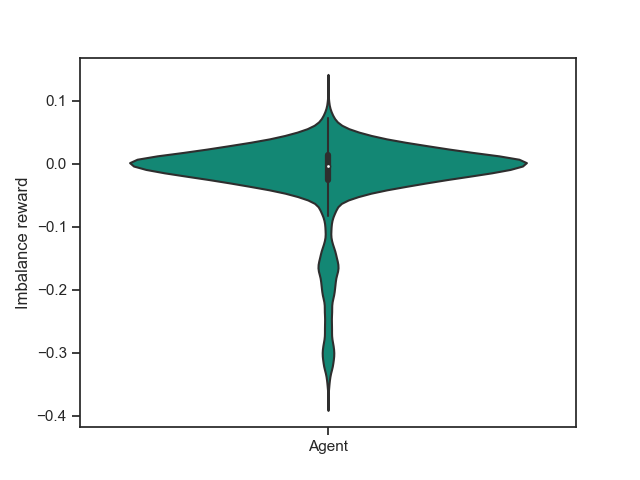
\includegraphics[height=8cm, width=12cm]{figures/config1_imbalance_reward.png}
    \caption[size = 9]{Violin plot of the imbalance reward given to the trained agent in a 500 episode simulation}
    \label{fig:discussion:config1_imbalance_reward}
\end{figure}

\section{Reinforcement learning algorithm}
This thesis has not tested different combinations of hyperparameters in the reinforcement learning algorithm. The default values for learning rate, neural network architecture and exploratory noise have been used. Naturally, performing a grid search to find optimal hyperparameters could boost the performance of the algorithm. Moreover, the training time consisted of 100 000 experiences, which is quite low considering that neural networks are used as functions approximators. One of the great features of neural network is that they continually can improve from new and unseen data. This was demonstrated in OpenAI's Dota Five reinforcement learning algorithm that has over 10 month real-time training \cite{openai_dota}. The relatively primitive behaviour of the trained agent could simply be a result of too little training time.

There have frequently been comments about the desired behaviour of the agent in this thesis. A legitimate question is whether a reinforcement learning algorithm is needed if one can say what the desired behaviour is. Why not simply increase consumption as much as possible in hours of peak solar production, and then decrease it in hours of peak demand, as this is always referred to as the desired behaviour? This can be a reasonable baseline to which the reinforcement algorithm can be compared. The trained agent has not been tested against a baseline in this thesis, but it is unlikely that it would beat it. The trained agent only managed to decrease consumption in hours of peak demand, and made the situation worse elsewhere. The simple baseline described would probably beat the trained agent because it would reduce the violations in periods of peak solar production as well. Admittedly, a reinforcement learning algorithm is perhaps somewhat overkill considering the action space, reward function and state representation used in this thesis. However, when factors such as price of flexibility, batteries, transformer control and user discomfort are included, the task quickly gets more complicated. It is no quick way to determine the desired behaviour of the agent in such a setup, where there are many more strategies. Still, it is necessary to inspect the deep deterministic policy gradient algorithm in a simpler task, where its behaviour can be analysed and discussed, and build on those experiences when expanding the setup further.

Deep deterministic policy gradient is an off-policy reinforcement learning algorithm, which means that it is capable of learning from the experiences of others. \texttt{stable\_baseline} offers a method that can clone an expert behaviour using supervised learning. Considering the large action space (16 independent variables), it would probably be beneficial to pretrain the agent using the experiences of a simple baseline that increases the consumption during peak solar production, and decreases it during peak demand. The probability that the agent by chance coordinates its action such that the consumption is increased at all loads is the same as flipping a coin 16 times and getting tails every time. Pretraining would guide the agent such that it does not have to spend all the training time to find the basic behaviour, but can start exploring strategies that are closely related to the baseline. 

\end{document}